You are perfectly familiar with solving equations involving an unknown variable $x$ and its powers. For example, $x=2$ solves $x^2-x-2=0$. We now study equations involving an unknown function and its derivatives. That is, we will be studying \emph{differential equations} (DEs). For example, $f(x)=e^{2x}$ solves $f''(x)-f'(x)-2f(x)=0$. Differential equations are difficult to solve, but it is important to keep in mind that checking whether a given function is a solution is more straightforward: you can verify that $f(x)=e^{2x}$ solves $f''(x)-f'(x)-2f(x)=0$ solely with your knowledge of differentiation. Which of $f(x)=e^{x}$ and $f(x)=e^{-x}$ is another solution of that differential equation?

Differential equations for functions of one variable are called \emph{ordinary differential equations} (ODEs), and for functions of several variables, they are called \emph{partial differential equations} (PDEs). Almost all natural processes obey differential equations, and they are therefore very important for physics and in engineering. However, besides classical physics and engineering applications such as describing the motion of objects, many other phenomena can be modelled with differential equations as well: for example, the growth of populations and the spread of diseases.

\begin{application}[Draining a tank]
~\\
\begin{minipage}{0.6\textwidth}
A water tank is being drained, and we are asked to find a formula for the height $h(t)$ of the water level as a function of time.

The behaviour of the height of the water level over time depends on how quickly water is leaving the tank, i.e. on the rate of change $h'(t)$. The problem now is the following: $h'(t)$ in turn depends on $h(t)$ -- for example, if the level is very high, the water pressure at the bottom of the tank will be very high and water will be forced out at a very high velocity.
\end{minipage} \hfill
\begin{minipage}{0.3\textwidth}
	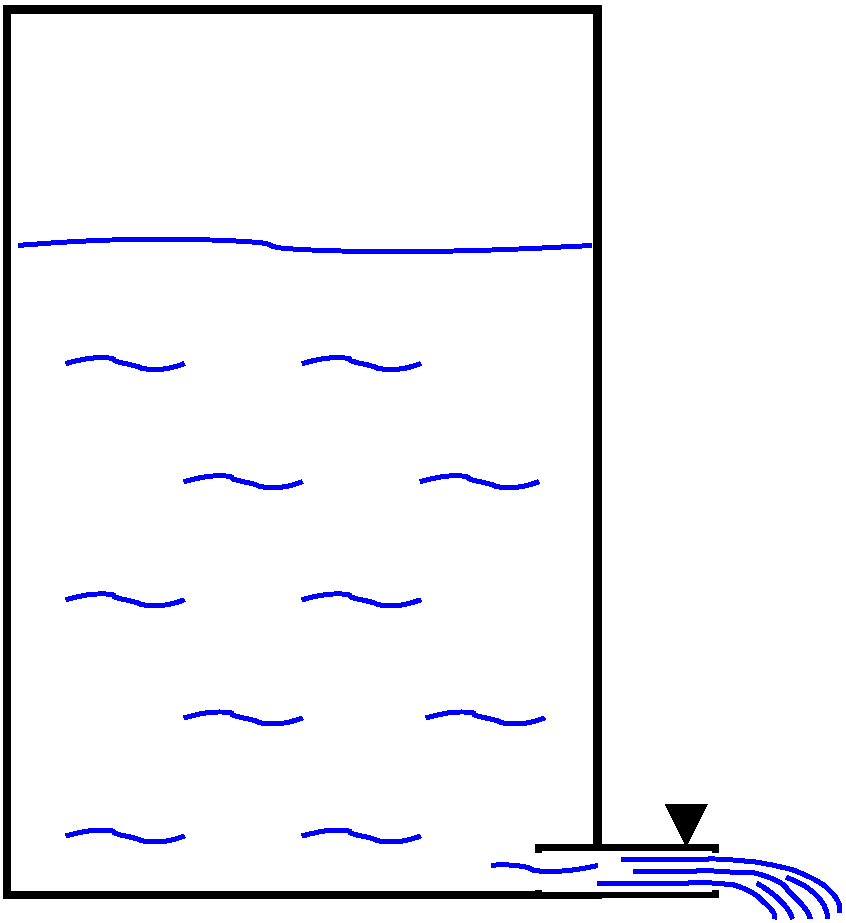
\includegraphics[width=0.9\textwidth]{./Figures/water_tank.pdf}
\end{minipage}

\medskip
From physical principles, one can derive the differential equation
\[ h'(t) = -\alpha \cdot \sqrt{h(t)} \]
for the height of the water level, where $\alpha$ is some positive constant that depends on the size of the tank and other parameters. This differential equation is known as Torricelli's law, and we will now learn how to solve it!
\end{application}


\section{First-Order Ordinary Differential Equations}
\label{sec:f-o}

\begin{definition}[ODEs, order, IVPs, solutions]
\label{def:f-o}
\begin{enumerate}[(i)]
	\item An \emph{ordinary differential equation (ODE)} is an equation involving an unknown function $y(x)$ and its derivatives
	\[ y'(x),\,y''(x),\,y'''(x),\,y^{(4)}(x),\,\dots,\,y^{(n)}(x) \]
	and other known functions of $x$.
	\item The order of the highest derivative appearing in an ordinary differential equation is called the \emph{order} of the ODE. For example, a first-order ODE is of the form
	\[ y' = f(x,y), \]
	where $f$ is a known function. The argument $x$ of $y$ is often omitted, but it is important to be aware that $y$ is a function.
	\item A first-order ODE together with an \emph{initial condition} of the form
	\[ y(x_0)=y_0, \]
	where the numbers $x_0,\,y_0$ are given, is called an \emph{initial-value problem (IVP)}.
	\item A function $y=y(x)$ that satisfies a given ODE is called a \emph{solution}. If $y$ contains parameters (constants) such that varying them covers all possible solutions to the ODE, then $y$ is called the \emph{general solution}. A solution that also satisfies given initial conditions is called a \emph{particular solution}. For now, i.e. until section~\ref{sec:pdes}, we can omit the specification 'ordinary'.
\end{enumerate}
\end{definition}

\begin{example}
\label{exple:first_de_exples}
\begin{enumerate}[(i)]
	\item The DE
	\[ y''(x)+4y(x)=0 \]
	has $y(x)=\sin(2x)$ as a solution. Indeed, we can check
	\begin{equation*}
	\begin{split}
	y(x) & =\sin(2x) \\
	\rightarrow \quad y'(x) & =2\cos(2x) \\
	\rightarrow \quad y''(x) & =-4\sin(2x) \\
	\rightarrow \quad y''(x) +4y(x) & = -4\sin(2x) + 4\sin(2x) = 0 \quad \text{\checkmark}.
	\end{split}
	\end{equation*}
	We will see later that the general solution is
	\[ y(x)=c_1\sin(2x)+c_2\cos(2x), \]
	which gives our guessed solution via the choice $(c_1,c_2)=(1,0)$ of constants.
	\item For the DE
	\[ y^{(4)} = 0, \]
	one can guess solutions $y(x)=1,\,y(x)=x^3,\,y(x)=2x^2-3x+5$, and hence the general solution
	\[ y(x) = Ax^3+Bx^2+Cx+D \]
	-- the polynomials of degree less than $4$.
\end{enumerate}
\end{example}

\begin{remark}
\label{rem:first_de_rems}	
\begin{enumerate}[(i)]
	\item As for integration: While solving DEs can be tricky, verifying solutions using differentiation is straightforward.
	\item Differential equations of the form
	\[ y'=f(x), \]
	i.e. when the function $f(x,y)$ in definition~\ref{def:f-o} (ii) does not depend on $y$, are the easiest to solve -- by integration:
	\[ y(x) = \itgr{}{}{f(x)}{x}. \]
	For example, the function $y(x)=\ln(x)+c$ solves the DE $y'=\rfrac1x$. We will refer to this type of DE as \emph{directly integrable}.
	\item The general solution of a $n$th-order DE usually contains $n$ constants. You can see that in the examples above. For directly integrable DEs, one can argue as follows: To solve
	\[ y^{(n)}=f(x), \]
	we integrate $f(x)$ $n$ times, obtaining a constant of integration each time. For this module, you can always work with the assumption that the general solution of a $n$th-order DE contains $n$ constants. Proving this for certain types of DEs -- it is not true for all DEs -- is beyond the scope of MTH1002.
	\item Our first non-trivial technique for solving ODEs is for those of the form
	\[ y'=h(x) \cdot g(y). \]
\end{enumerate}
\end{remark}

\subsection{Separable DEs}

\begin{example}
\begin{enumerate}[(i)]
	\item To solve the DE
	\[ y' = x \cdot y, \]
	we first write it as
	\[ \Df{y}{x} = x \cdot y \]
	and then \emph{separate variables}. That is, bring all expressions with an $x$ on one side and all expressions with $y$ on the other side. For that, we treat $dx$ like a number and 'multiply' the DE by it. Integrating gives
	\begin{equation}
	\label{eq:first_sop}
	 \itgr{}{}{\frac{1}{y}}{y} = \itgr{}{}{x}{x},
	\end{equation}
	which leads to
	\[ \ln\abs{y} = \frac{x^2}{2} + c_1 \qquad (c_1\in\mathbb{R}). \]
	Applying $\exp(.)$ on both sides gives
	\[ \abs{y} = \e^{\rfrac{x^2}{2}+c_1} = \e^{\rfrac{x^2}{2}}\,\e^{c_1} = c_2\, \e^{\rfrac{x^2}{2}} \qquad (c_2\in\mathbb{R}^+),\]
	where we let $c_2=\e^{c_1}$. Now, the absolute value on the left is either a factor of $+1$ or $-1$, depending on whether $y$ is positive or negative. Absorbing this potential negative sign into the constant, we have
	\[ y=c_3\,\e^{\rfrac{x^2}{2}} \qquad (c_3\in\mathbb{R}\backslash\{0\}). \]
	Even though $c_3 \not= 0$ is excluded, we note that a constant of $0$ works as well: Then we have $y(x)=0$ and 
	\[ y'(x) = 0 = x \cdot y. \]
	Hence we include the possibility $c=0$ and find the general solution to be
	\[ y(x) = c\,\e^{\rfrac{x^2}{2}} \qquad (c\in\mathbb{R}). \]
	
	Note that after~\eqref{eq:first_sop}, one should have stated that the function $y(x)$ can not have any zeros, since otherwise the integrand on the left-hand side would not be defined. Hence one solves the DE only on intervals on which $y$ is either always positive or always negative, and considers the case of $y$ having a zero separately. If $y(x_0)=0$, then $y'(x_0)=0$ by the original DE, and this suggests that the constant function $y(x)=0$ is a solution. Now, for the remaining cases, $y$ is either always positive or always negative, which allows to absorb the potential negative from $\abs{y}$ into the constant $c_2$. However, we will not always discuss the solution of DEs and the ranges of any constants involved that carefully. For example, in the next computation we might change the meaning of constants from one line to the next without explicitly renaming them.
	\item Solve the IVP
	\[ \left\{ \begin{split} 1+xyy' & = y^2+yy' \\ y(0) & = -\rfrac12. \end{split} \right. \]
	{\it Sol.:}
	\begin{equation*}
	\begin{split}
	\rightarrow & \quad (xy-y)\Df{y}{x} 
	= y^2-1 \quad \stackrel{\text{sep. of var.}}{\rightarrow} \quad
	\itgr{}{}{\frac{y}{y^2-1}}{y} = \itgr{}{}{\frac{1}{x-1}}{x} \\
	\stackrel{u=y^2-1}{\rightarrow} & \quad \frac12 \itgr{}{}{\frac1u}{u} = \ln\abs{x-1}+c \quad
	\stackrel{\text{integrate}}{\rightarrow} \quad \frac12\ln\abs{y^2-1} = \ln\abs{x-1} + c \\ 
	\stackrel{\cdot 2}{\rightarrow} & \quad \ln\abs{y^2-1} = \ln(x-1)^2+c \quad 
	\stackrel{\exp(.)}{\rightarrow} \quad \abs{y^2-1} = \e^{\ln(x-1)^2+c} \\
	\stackrel{\text{as in (i)}}{\rightarrow} & \quad y^2-1 = c\,(x-1)^2 \quad
	\rightarrow \quad y^2+c\,(x-1)^2=1.
	\end{split}
	\end{equation*}
	This is the general solution of the DE, but it is in implicit form, i.e. not solved for $y$ (it is not an explicit formula for $y(x)$). Next, we use the given initial data $(x_0,y_0)=(0,-\rfrac12)$:
	\[ \left(-\frac12\right)^2+c\,(0-1)^2 = \frac14+c\stackrel{!}{=} 1, \]
	which gives $c=\rfrac34$ and the explicit solution
	\[ y=\pm \sqrt{1-\rfrac34\,(x-1^2)}. \]
	For the particular solution to the given IVP, it remains to decide between $+$ and $-$. We choose
	\[ y(x) = -\sqrt{1-\rfrac34\,(x-1^2)} \]
	-- why not the positive solution\footnote{Check the initial condition for both possible choices.}?
\end{enumerate}
\end{example}

\begin{remark}
\label{rem:sov}
\begin{enumerate}[(i)]
	\item The implicit general solution $y^2+c\,(x-1)^2=1$ in (ii) describes an ellipse for $c>0$ (centred at $(1,0)$; a circle for $c=1$), a hyperbola for $c<0$, and a pair of horizontal lines for $c=0$.
	\item Next we study DEs of the form
	\[ \Df{y}{x} = f(x,y) = F\left(\rfrac{y}{x}\right),\]
	which we call \emph{homogeneous-type} and which can be transformed into separable DEs. A DE is homogeneous-type if 
	\[ f(\lambda x,\lambda y) = f(x,y) \qquad \text{for all~} \lambda\not=0. \]
\end{enumerate}
\end{remark}


\subsection{Homogeneous-Type}

\begin{example} Solve
	\[ \Df{y}{x}=\frac{x^2+y^2}{xy}. \]
{\it Sol.:} This DE is not separable. The expression on the right is invariant under replacing $x$ and $y$ with $\lambda x$ and $\lambda y$, respectively, so the DE is of homogeneous type. We solve it as follows:
\begin{equation}
\label{eq:homog1}
\Df{y}{x} = \frac{x^2\left( 1+\rfrac{y^2}{x^2} \right)}{x^2\:\rfrac{y}{x}}
= \frac{1+(\rfrac{y}{x})^2}{\rfrac{y}{x}} = F\left(\rfrac{y}{x}\right),
\end{equation}
where $F$ is the single-variable function defined by
\[ F(t) = \frac{1+t^2}{t}. \]
Set $t=\rfrac{y}{x}$, and note that it is a function of $x$: $t=t(x)$. Next, we find the relation between $y'$ and $t'$:
\begin{equation}
\label{eq:homog2}
 \Df{y}{x} = \Df{}{x}(x \cdot t ) = xt'+t.
\end{equation}
Combining \eqref{eq:homog1} and \eqref{eq:homog2}, we obtain a DE for $t(x)$:
\[ x\,t'+t=\frac{1+t^2}{t} \quad \rightarrow \quad x\,t'=\frac{1+t^2}{t}-t=\frac{1}{t}. \]
Writing this as
\[ x\,\Df{t}{x} = \frac{1}{t}, \]
we see that it is a separable DE, which we solve with the steps from the previous section:
\[ \itgr{}{}{t}{t} = \itgr{}{}{\frac{1}{x}}{x} \quad \rightarrow \quad
t^2 = \ln x^2+c = \left( \frac{y}{x} \right)^2, \]
which gives the general solution
\[ y(x) = \pm \, x \, \sqrt{\ln x^2+c}\,. \]
\end{example}

\subsection{Linear DEs}

\begin{definition}[Linear First-Order ODEs, Homogeneity]
\begin{enumerate}[(i)]
	\item A first-order ODE of the form
	\[ y'+p(x)\,y=r(x) \]
	is called \emph{linear}.
	\item It is further called \emph{homogeneous} if $r(x)=0$, and \emph{inhomogeneous} otherwise.
\end{enumerate}
\end{definition}

\begin{remark} Multiplying this DE by its \emph{integrating factor}
	\[ h(x):=\e^{P(x)}, \]
	where $P$ is any antiderivative of $p$, we obtain
	\[ h\,r =h\,y'+h\,p\,y= h\,y'+h'\,y = (h\,y)', \]
	which can be solved by integrating both sides:
	\[ h(x) \cdot y(x) = \itgr{}{}{h(x) \cdot r(x)}{x}. \]
\end{remark}

\begin{example}
\begin{enumerate}[(i)]
	\item Solve \[ y' +\frac{5}{x}\,y=\cos\left( x^6 \right).\]
	{\it Sol.:} The DE is linear, and the integrating factor 
	\[ h(x) = \e^{\itgr{}{}{\rfrac{5}{x}}{x}} = \e^{5\ln x} = x^5. \]
	Note that the constant of integration was omitted in the integration of $p(x)$ -- that is because the method using the integrating factor works for any antiderivative, and hence one can choose the easiest one: the antiderivative with $c=0$. Next, we find
	\[ x^5\,y=\itgr{}{}{x^5\,\cos\left(x^6\right)}{x} \stackrel{u=x^6}{=} \dots 
	= \frac16\left( \sin\left( x^6 \right) + c \right). \]
	Finally, dividing by the integrating factor gives the solution:
	\[ y(x)=\frac{\sin\left(x^6\right)+c}{6x^5}\,. \]
	\item Solve the IVP
	\[ \left\{ \begin{split}
	(1+x^2)y'-2xy&=1+x^2 \\ y(1)&=6.
	\end{split} \right. \]
	{\it Sol.:} First bring the DE in the correct form:
	\[ y'-\frac{2x}{1+x^2}y=1.\]
	Now one can read off the antiderivative $P(x)=-\ln(1+x^2)$ of $p(x)$. This gives the integrating factor
	\[ h(x)=\e^{-\ln(1+x^2)}=\frac{1}{1+x^2}, \]
	and therefore the general solution
	\[ y(x) = (1+x^2) \itgr{}{}{\frac{1}{1+x^2} \cdot 1}{x} 
	= (1+x^2)( \arctan x + c ).\]
	The initial condition gives
	\[ 6=(1+1^2)\left(\frac{\pi}{4}+c\right) \quad \rightarrow \quad
	y(x)=(1+x^2)\left( \arctan x + 3-\frac{\pi}{4} \right). \]
\end{enumerate}
\end{example}

\begin{application}[Logistic growth]
\texttt{\ldots}
\end{application}

\begin{exercise}
\begin{enumerate}[(i)]
	\item Work through the first-order DEs on the tutorial sheet for chapter~4.
	\item Letting $\alpha=1$ and $h(0)=100$, solve the differential equation for the water tank from the beginning of this chapter. Plot your solution -- does it make sense\footnote{Initially, it does not make sense, but setting the solution equal to $0$ from a certain $t_0$ on, one obtains a function for the water level $h(t)$ that does agrees with how one would imagine a tank to drain.}? How long does it take for the tank to drain\footnote{$20$ seconds.}?
	\item Solve\footnote{$y(x) \approx x \cdot \text{arcsin} ( \ln x + 0.866 )$,
	but you should obtain the constant exactly.}
	\[ xy'=y+x\sec\left(\frac{y}{x}\right), \quad y(1)=\frac{\pi}{3}.\]
	\item Solve\footnote{$y(x)=\frac{\sin^2x}{\cos x}$.}
	\[ y' = y \tan x + \sin x, \quad y(0)=0. \]
	\item Prove the statement from remark~\ref{rem:sov} (ii): Let $f(x,y)$ be a continuous function on $\mathbb{R}^2\backslash\{(0,0)\}$, i.e. $f$ is defined on the $xy$-plane without the origin $(x,y)=(0,0)$. There exists a single-variable function $F(t)$ such that 
	\[ f(x,y)=F(\rfrac{y}{x}) \]
	for any $x\not=0$, if and only if\footnote{Perhaps stating this more formally makes it more clear what needs to be done: Let $f=f(x,y)$ be continuous on $\mathbb{R}^2\backslash\{(0,0)\}$. Then
	\[ \exists \: F=F(t): f(x,y)=F(\rfrac{y}{x}) \: \forall x\not=0
	\: \Longleftrightarrow \: f(x,y)=f(\lambda x, \lambda y) \: \forall \lambda\not=0.
	\] The direction ``$\Longrightarrow$'' is the easier one. The case $x=0$ causes some extra work -- one can use continuity for that -- but it would be alright to skip this technicality.}
	\[ f(x,y) = f(\lambda x, \lambda y) \qquad \text{for all~}\lambda\not=0.\]
\end{enumerate}
\end{exercise}


\section{Linear Ordinary Differential Equations of Higher Order}
\label{sec:s-o}

\begin{definition}[Second-Order Linear ODEs]
	The standard form for a \emph{second-order linear ODE is}
	\[ y''+p(x)y'+q(x)y=r(x). \]
	A LODE is called homogeneous if $r(x)=0$, inhomogeneous otherwise.
\end{definition}

\begin{remark}
\label{rem:s-o_lode}
\begin{enumerate}[(i)]
	\item If we set
	\[ L[y]=y''+p(x)y'+q(x)y, \]
	the DE reads $L[y]=r(x)$. Here, $L$ is a \emph{differential operator} -- it takes a function as input and outputs a function. For example, the differential operator
	\[ \wtd{L}=7\Df{}{x} \]
	would map the input $x^2$ to $14x$.
	\item For LODEs: If $y_1,\,y_2$ are functions and $\alpha,\,\beta$ constants, then
	\[ L[\alpha y_1 + \beta y_2] = \alpha L[y_1] + \beta L[y_2]. \]
	\item If $y_1$ and $y_2$ are solutions to a homogeneous s-o LODE and they are \emph{linearly independent} (i.e. $y_2 \not= c \cdot y_1$), then
	\[ y(x) = c_1 y_1(x) + c_2 y_2(x) \]
	is the general solution.
	\item However, the previous statement, (iii), is not true in the inhomogeneous case: If
	\[ L[y_1] = r(x) \quad \text{and} \quad L[y_2] = r(x), \]
	then
	\[ L[y_1+y_2] = L[y_1] + L[y_2] = 2r(x), \]
	that is, $y_1+y_2$ does not satisfy $L[y]=r(x)$ (unless $r(x)=0$, which is the homogeneous case (iii)).
	\item The following technique allows us to find the general solution if one solution is known or can be guessed.
\end{enumerate}
\end{remark}

\subsection{Reduction of Order}

\begin{example}
Given the solution $y_1(x)=x$ of 
\[ x^2y''+xy'-y=0, \]
find $y_2$ and hence the general solution. \\
{\it Sol.:} First, one should verify that $y_1$ really is a solution:
\[ x^2y_1''+xy_1'-y_1=x^2 \cdot 0 + x \cdot 1 - x = x-x = 0 \quad \text{\checkmark}. \]
Now make the ansatz $y(x)=v(x) \cdot y_1(x)$, or, abbreviated, \[y=vy_1.\] The idea behind this ansatz is: the other solutions should be structurally similar to $y_1$, as they satisfy the same differential equation. From this viewpoint, it seems possible that using the knowledge of $y_1$ and analysing its ratio with other solutions might reduce the complexity of the problem. We have
\[ y=vy_1,\quad y'=v'y_1+vy_1', \quad y''=v''y_1+2v'y_1'+vy_1'', \]
and therefore
\begin{equation*}
\begin{split}
L[y] & = L[vy_1] = x^2 \cdot \left[ v''y_1+2v'y_1'+vy_1'' \right]
+ x \cdot \left[ v'y_1+vy_1' \right] - \left[ vy_1 \right] \\
& = x^2v''y_1+2x^2v'y_1'+xv'y_1+v \cdot
\underbrace{\left[ x^2y_1''+xy_1'-y_1 \right]}_{=L[y_1]=0} \\
& = x^2v''y_1+2x^2v'y_1'+xv'y_1+v \cdot 0 \qquad (\text{now use~} y_1=x,\,y_1'=1,\,y_1''=0) \\
& = x^3v''+3x^2v' \stackrel{w=v'}{=} x^3w'+3x^2w \stackrel{!}{=} 0.
\end{split}
\end{equation*}
That is, if $w=w(x)$ satisfies the first-order LODE
\[ x^3w'+3x^2w = 0, \]
then $y=vy_1$ will satisfy the original second-order LODE. We find
\begin{equation*}
\begin{split}
w(x) &= \frac{\alpha}{x^3}, \\
v(x) &= -\frac{\alpha}{2}x^{-2} + \beta, \\
y(x) &= \beta x - \frac{\alpha}{2} \frac{1}{x},
\end{split}
\end{equation*}
where $\alpha, \beta \in \mathbb{R}$, and, after renaming the constants,
\[ y(x) = c_1 \cdot x + c_2 \cdot \frac{1}{x}. \]
This is the general solution of the DE, and it is in the form mentioned in remark~\ref{rem:s-o_lode} (iii), with $y_2=\rfrac{1}{x}$.
\end{example}

\begin{remark}
We recommend writing out $L[y]=L[vy_1]=\dots$ as above, rather than using the formula for $y_1$, which is already known at this point. Then, \emph{after} the term $v \cdot L[y_1]$ has dropped out of the computation, one can substitute in the formula for $y_1$ and its derivatives. Using the formula for $y_1$ from the beginning, i.e. $L[y]=L[v \cdot x]=\dots$ in this case, would often make the computation more complicated, e.g. if $y_1$ is a rational function with bulky derivatives. 
\end{remark}

\subsection{Constant-Coefficient Homogeneous}
\label{sec:cch}

\begin{remark} Consider the second-order LODE
\label{rem:cch}
	\begin{equation}
	\label{eq:char_eq1}
		L[y] = y''+py'+qy = 0,
	\end{equation} 
	where $p,\,q$ are \emph{constants}, not functions of $x$. Making the ansatz
	\[ y(x) = \e^{\lambda x}, \]
	we find
	\[	0  \stackrel{!}{=} L[\e^{\lambda x}]
	= \Ddf{}{x} \left( \e^{\lambda x} \right) +
	p\,\Df{}{x} \left( \e^{\lambda x} \right) + q\,\e^{\lambda x} 
	= \e^{\lambda x}\left(\lambda^2+p\,\lambda+q\right). \]
	That is, if $\lambda$ satisfies the \emph{characteristic equation} (or \emph{auxiliary equation})
	\begin{equation}
	\label{eq:char_eq2}
		\lambda^2+p\,\lambda+q = 0,
	\end{equation}
	then $y=\e^{\lambda x}$ is a solution of~\eqref{eq:char_eq1}. The solutions of~\eqref{eq:char_eq2} are
	\[ \lambda_{1/2} = \frac{-p\pm\sqrt{p^2-4q}}{2}, \]
	and we now have to consider three cases:
	\begin{enumerate}[(I)]
		\item If~\eqref{eq:char_eq2} has two distinct real solutions $\lambda_1$ and $\lambda_2$ -- this happens when $p^2-4q>0$ -- then we have solutions
		\[ y_1(x) = \e^{\lambda_1 x}, \qquad y_2(x) = \e^{\lambda_2 x}, \]
		of~\eqref{eq:char_eq1}. From earlier theory, we conclude that the general solution is
		\[ y(x) = c_1\,\e^{\lambda_1 x} + c_2\,\e^{\lambda_2 x}.\]
		\item If~\eqref{eq:char_eq2} has one real solution $\lambda$ (i.e. a double root, $\lambda_1=\lambda_2$) -- this happens when $p^2-4q=0$ -- then we have solutions
		\[ y_1(x) = \e^{\lambda x}, \qquad y_2(x) = x\,\e^{\lambda x}. \]
		That $y_1$ is a solution follows again from $\lambda$ solving the characteristic equation, and $y_2$ is obtained via reduction of order. Note that $\lambda=-\rfrac{p}{2}$ in this case. The general solution is
 		\[ y(x) = c_1\,\e^{\lambda x} + c_2\,x\,\e^{\lambda x}. \]
		\item If~\eqref{eq:char_eq2} has no real solutions -- this happens when $p^2-4q<0$ -- then it has complex solutions 
		\[ \lambda_{1/2} = a \pm ib \qquad (a,b\in\mathbb{R}), \]
		and the solutions to the differential equation are
		\[ y_1(x) = \e^{ax}\cos(bx), \qquad y_2(x) = \e^{ax}\sin(bx). \]
		The derivation of this is outlined in the exercises below. The general solution is
		\[ y(x) = \e^{ax}\left[ c_1\cos(bx)+c_2\sin(bx) \right]. \]
\end{enumerate}
\end{remark}

\begin{definition}[IVPs and BVPs]
	For a second-order ODE, $L[y] = r(x)$,
	the system of equations
	\begin{equation*}
	\left\{
	\begin{split}
L[y] &= r(x) \\ y(a) &= A \\ y'(a) &= B 
	\end{split}\right.
	\end{equation*}
	is called an \emph{initial-value problem} (IVP). A system of the form
	\begin{equation*}
	\left\{
	\begin{split}
L[y] &= r(x) \\ y(a) &= A \\ y(b) &= B 
	\end{split}\right.
	\end{equation*}
	is called an \emph{boundary-value problem} (BVP).
\end{definition}

\begin{example}
\label{expl:bvps_ivps}
\begin{enumerate}[(i)]
	\item
	\[ \left\{ 
	\begin{split}
		y''-3\,y'+\rfrac{9}{4}\,y & = 0 \\ 
		y(0) & = 0 \\ y\left(\rfrac{2}{3}\right) & = 1
	\end{split}
	\right.\]
	{\it Sol.:} We first consider the DE only, which is second-order, linear, and homogeneous with constant coefficients. Its characteristic equation is
	\[ 0 = \lambda^2-3\lambda+\frac94 = (\lambda-\rfrac32)(\lambda-\rfrac32), \]
	which has the double root $\lambda=\rfrac32$, i.e. we have case (II) from the discussion above. This value of $\lambda$ implies that the general solution is
	\[ y(x) = c_1\,\e^{\rfrac32\,x} + c_2\,x\,\e^{\rfrac32\,x}, \]
	and it remains to determine the constants so that $y$ satisfies the given boundary conditions:
	\[ \begin{split}
	0 \stackrel{!}{=} y(0) & = c_1\cdot1 +c_2\cdot0\cdot1 = c_1 \\
	1 \stackrel{!}{=} y\left( \rfrac23 \right) 
		& = c_1 \cdot \e + c_2 \cdot \rfrac23 \cdot \e = \rfrac{2\e}{3}\,c_2,
	\end{split}\]
	which leads to the particular solution 
	\[ y(x) = \frac{3x}{2\e}\,\e^{\rfrac23\,x}. \]
	\item
		\[ \left\{ 
	\begin{split}
			y''-y'+\rfrac{17}{4}\,y & = 0 \\ 
			y(0) & = 0 \\ y'(0) & = 10
	\end{split}
	\right.\]
	{\it Sol.:} 
	The characteristic equation is 
	\[ \lambda^2-\lambda +\frac{17}{4} = 0, \]
	which has solutions
	\[ \lambda_{1/2} = \frac{-(-1)\pm\sqrt{(-1)^2-4 \cdot \rfrac{17}{4}}}{2}
	= \frac12 \pm \frac{\sqrt{-16}}{2} = \frac12 \pm i \cdot 2, \]
	and therefore leads to the general solution
	\[ y(x) = \e^{\rfrac{x}{2}}\left( c_1\cos(2x) + c_2\sin(2x) \right). \]
	In order to find the solution of the IVP, we need to set the values of $y$ and $y'$ at $x=0$ equal to the given values. Therefore, $y'(x)$ needs to be found:
	\[ y'(x) = \frac12\e^{\rfrac{x}{2}}\left( c_1\cos(2x) + c_2\sin(2x) \right)
	+\e^{\rfrac{x}{2}}\left(-2c_1\sin(2x) + 2c_2\cos(2x) \right).\]
	Now we can solve for the constants:
	\[ \left\{ \begin{split}
	0=y(0)&=\e^0 (c_1\cos 0 + c_2\sin 0) = c_1 \\
	10=y'(0)&=\rfrac12\,\e^0(c_1\cos 0 + c_2\sin 0)
	+ \e^0 (-2c_1\sin 0 + 2c_2\cos 0)=\rfrac{1}{2}\,c_1+2c_2,
	\end{split}\right.\]
	which gives $c_1=0,\,c_2=5$ and hence
	\[ y(x) = 5\,\e^{\rfrac{x}{2}}\sin(2x). \]
	\item
	\[\left\{ \begin{split}
	y''+y'-6y &= 0 \\ y(0) &= 1 \\ y'(0) &= 12
	 \end{split}\right.\]
	{\it Sol.:} 
	\[ y(x) = 3\,\e^{2x}-2\,\e^{-3x}\]
\end{enumerate}
\end{example}

\begin{remark}
\begin{enumerate}[(i)]
	\item At the beginning of this chapter, in remark~\ref{rem:first_de_rems}, it was stated that the general solution of a $n$th-order DE contains $n$ constants. From this, one can deduce that it takes $n$ conditions to specify a particular solution -- this agrees with the examples we have seen so far: one condition in section~\ref{sec:f-o} and two conditions (either IVP or BVP) for the second-order DEs in the previous example.
	\item The difference between an IVP and an BVP can be illustrated as follows. Many natural processes obey second-order differential equations, and the motion of objects is a prominent example. Suppose a ball is kicked vertically in the air, and you are shown a snapshot of it. That is, you are given the height at a certain time, $h(t_1)$. From this, you cannot say what will happen next -- for example, you do not know whether the ball was on its way up or down when the picture was taken. However, if you are given a second piece of information, you can -- with your knowledge from this module -- determine the exact trajectory $h(t)$ of the ball. This second piece of information could be the velocity $h'(t_1)$ of the ball ($\rightarrow$ IVP; how fast and in which direction was it moving when the picture was taken) or the position at some other specified time ($\rightarrow$ BVP; e.g., another snapshot, taken exactly one second later).
	\item The method of using the characteristic equation remains applicable for LODEs of higher orders -- however, then the characteristic equation will be of higher order as well, and it might therefore not be readily solvable. Sometimes, one is able to guess one solution and then reduce its order, cf. the next example.
\end{enumerate}
\end{remark}

\begin{example}
\[ y''' - \frac12 \, y'' -\frac{41}{2} \, y' + 35 \, y = 0 \]
{\it Sol.:} The characteristic equation is 
\[ \lambda^3 - \frac12 \, \lambda^2 -\frac{41}{2} \, \lambda + 35 = 0, \]
and after some experimentation, one finds the solution $\lambda = 2$, since $8-2-41+35=0$.  This means that $(\lambda-2)$ is a factor of the cubic expression on the left -- dividing by it (long division of polynomials), we obtain
\[ 0 = \lambda^3 - \frac12 \, \lambda^2 -\frac{41}{2} \, \lambda + 35 
= (\lambda-2)\left( \lambda^2+\frac32\lambda-\frac{35}{2} \right) = (\lambda-2)(\lambda-\rfrac{7}{2})(\lambda+5),\]
and therefore the general solution
\[ y(x) = c_1\,\e^{2x} + c_2\,\e^{\rfrac{7}{2}x} + c_3\,\e^{-5x}. \]
\end{example}

\subsection{Constant-Coefficient Inhomogeneous}

\begin{remark}
\begin{enumerate}[(i)]
	\item The steps for solving an \emph{inhomogeneous} linear second-order DE with constant coefficients, 
	\[ L[y] = y''+py'+qy = r(x), \qquad \qquad p,\,q\in\mathbb{R},\]
	are:
	\begin{enumerate}[(1)]
		\item Solve the corresponding homogeneous DE, $L[y] = 0$. Its general solution is called the \emph{complementary function}:
		\[ y_{CF} = c_1y_1+c_2y_2. \]
		\item Find one solution of the inhomogeneous DE, $L[y]=r(x)$. This solution is denoted $y_{PI}$ and called the \emph{particular integral}. Finding $y_{PI}$ will be discussed below.
		\item The general solution of the inhomogeneous DE is
		\[ y = y_{CF} + y_{PI} = c_1y_1+c_2y_2 + y_{PI}. \]
		\item If the DE was given as an IVP or a BVP, i.e. with two additional conditions, then determine the constants in the general solution (3) so that the resulting function satisfies those conditions. This function is the solution to the IVP/BVP.
	\end{enumerate}
	\item Let us check whether the function from step (3) above really is the general solution of $L[y]=r(x)$: The function
	\[ y = y_{CF} + y_{PI} = c_1y_1+c_2y_2 + y_{PI} \]
	does contain two constants -- as we expect for the general solution of a second-order DE -- and
	\begin{equation*}
	\begin{split}
	L[y] = L[c_1y_1+c_2y_2 + y_{PI}] &= c_1L[y_1] + c_2L[y_2]+L[y_{PI}] \\ 
	&= c_1 \cdot 0 + c_2 \cdot 0 + r(x) = r(x) \quad \text{\checkmark}.
	\end{split}
	\end{equation*}
\end{enumerate}
\end{remark}

\begin{example}
Solve the IVP
\[ \left\{ \begin{split}
y''-y'-12y & = \e^{2x} \\ y(0) & = -2 \\ y'(0) & = 2
\end{split} \right. .\]
{\it Sol.:}
\begin{enumerate}[(1)]
	\item First we consider the homogeneous version of the DE,
	\[ y''-y'-12y = 0. \]
	Its characteristic equation is
	\[ 0 = \lambda^2-\lambda-12 = (\lambda-4)(\lambda+3), \]
	and it leads to the two solutions 
	\[ y_1(x) = \e^{4x}, \qquad y_2(x) = \e^{-3x}, \]
	of the homogeneous DE. Hence the complimentary function is
	\[ y_{CF}(x) = c_1 \, \e^{4x} + c_2 \, \e^{-3x}. \]
	\item Next, we need one solution of the inhomogeneous DE, the particular integral, $y_{PI}$. The idea is to make an ansatz containing parameters for it and then substitute it into $L[y]=\e^{2x}$ to determine those parameters. Choosing the correct form for $y_{PI}$ is key:
	\begin{enumerate}[{Attempt} 1:]
		\item Take $y_{PI}(x)=\sqrt{Ax^2+Bx+C}$. However, thinking about the action of the operator $L$, we see that 
		\[ \begin{split}
L[y_{PI}]&=L\left[\sqrt{Ax^2+Bx+C}\right] \\
&=\Ddf{}{x}\left[\sqrt{Ax^2+Bx+C}\right]-\Df{}{x}\left[\sqrt{Ax^2+Bx+C}\right] \\
& \qquad \quad \qquad \qquad \qquad \qquad -12\left[\sqrt{Ax^2+Bx+C}\right] = \dots
		\end{split}  \]
		will not lead to an expression that can be made equal to $\e^{2x}$ by making suitable choices for $A,\,B,\,C$.
		\item For $y_{PI}(x) = A\cos x +B\sin x$, application of $L$ will give a combination of trigonometric functions $\cos x$ and $\sin x$, not $\e^{2x}$.
		\item The previous attempts suggest that one should make an ansatz of the same form as the inhomogeneity $r(x)$. Hence try $y_{PI}(x) = A\e^{2x}$:
		\[ L[y_{PI}]=L\left[ A\e^{2x} \right] 
		= A \left[ 4 \e^{2x} - 2 \e^{2x} - 12 \e^{2x} \right] 
		= A (-10) \e^{2x} \stackrel{!}{=}\e^{2x},\]
		and therefore $A=\rfrac{-1}{10}$,
		\[ y_{PI}(x) = \frac{-1}{10}\e^{2x}. \]
		General advice on how to make the ansatz for the particular integral will be given below.
	\end{enumerate}
	\item The general solution of the original inhomogeneous DE is
			\[ y = y_{CF} + y_{PI} = c_1\,\e^{4x}+c_2\,\e^{-3x} - \frac{1}{10}\,\e^{2x}. \]
	\item The initial conditions give rise to the system 
	\[ \left\{ \begin{split}
		-2 = y(0) & = c_1+c_2-\rfrac{1}{10} \\
		2 = y'(0) & = 4c_1-3c_2-\rfrac{2}{10},
	\end{split} \right. \]
	which has solutions $c_1=-\rfrac12,\,c_2=-\rfrac{7}{5}$. This gives the solution to the IVP as
	\[ y = -\frac12\,\e^{4x}-\frac{7}{5}\,\e^{-3x} - \frac{1}{10}\,\e^{2x}. \]
\end{enumerate}
\end{example}

\begin{remark}
\label{rem:inhomog}
\begin{enumerate}[(i)]
	\item The following table and remarks should help you make the ansatz for the particular integral:
	\begin{center}
		\begin{tabular}{ | c | c | }
			Right-hand side $r(x)$ & Ansatz for $y_{PI}$ \\ \hline \hline
			polynomial of degree $m$: & polynomial of degree $m$: \\ 
			$\alpha_m x^m + \dots \alpha_1 x + \alpha_0$ 
			& $A_m x^m + \dots A_1 x + A_0$ \\ \hline
			exponential: & exponential: \\ 
			$\alpha\e^{\lambda x}$ & $A\e^{\lambda x}$ \\ \hline
			comb. of trig. functions: & comb. of trig. functions: \\
			$\alpha \cos(\lambda x) + \beta \sin(\lambda x)$ &
			$A\cos(\lambda x) + B\sin(\lambda x)$ \\ \hline 
			\ldots & \ \ldots \\
			(e.g.: comb. of hyp. trig. fcns & comb. of hyp. trig. fcns) \\ \hline
			a sum of any of the above: & find $y_{PI,j}$ for each $r_j$ and then: \\
			$r(x) = r_1(x) + \dots + r_k(x)$ &
			$y_{PI} = y_{PI,1} + \dots + y_{PI,k}$  \\ \hline
		\end{tabular}
	\end{center}
	Here it is important to always have full generality on the ansatz side: E.g., if $r(x)=2\sin(3x)$, i.e. there is no $\cos(3x)$ term in the inhomogeneity, one still needs $y_{PI}=A\cos(3x) + B\sin(3x)$ rather than an ansatz with a sine term only. If, for example, $r(x)=\sin(5x)+\cos(2x)$, the rule in the middle row of the table needs to be applied twice -- once for $\lambda=5$ and once for $\lambda=2$ -- and the outcomes are then to be combined as in the last row. If you have written out the ansatz $y_{PI}$ based on $r(x)$, but this $y_{PI}$ happens to already be a solution to the homogeneous version of the DE, then multiply it by~$x$.
	\item The linearity of the ODE is crucial for the above approach of finding all solutions of the homogeneous DE and then adding one solution of the inhomogeneous DE. Let us compare this to another linear situation: An inhomogeneous linear equation for the variables $x,\,y,\,z$: Solve 
	\begin{equation}
	\label{eq:plane}
	x+2y-5z = 2. 
	\end{equation}
	{\it Sol.:} 
	\begin{enumerate}[(1)]
		\item For the homogeneous version of the equation,
		\[ x+2y-5z = 0, \]
		we can find the two linearly independent (cf. \ref{def:li} for the general definition of this term) solutions
		\[ v_1 = \begin{bmatrix} 5 \\ 0 \\ 1\end{bmatrix}, \qquad 
		   v_2 = \begin{bmatrix} 0 \\ 5 \\ 2\end{bmatrix} \]
		and hence the general solution 
		\[ v_{CF} = c_1 \begin{bmatrix} 5 \\ 0 \\ 1\end{bmatrix}
		+ c_2 \begin{bmatrix} 0 \\ 5 \\ 2\end{bmatrix}. \]
		\item We now just need a single vector that satisfies the inhomogeneous equation~\eqref{eq:plane}. For example, 
		\[ v_{PI} = \begin{bmatrix} 2 \\ 0 \\ 0 \end{bmatrix}, \]
		as
		\[ \begin{bmatrix}	1 & 2 & -5 \end{bmatrix}
		\begin{bmatrix} 2 \\ 0 \\ 0	\end{bmatrix} = 2 \quad \text{\checkmark} \]
		(the entries of the row vector are the coefficients of \eqref{eq:plane}).
		\item The general solution of the inhomogeneous equation is
				\[ v = \begin{bmatrix} 2 \\ 0 \\ 0 \end{bmatrix} +
				c_1 \begin{bmatrix} 5 \\ 0 \\ 1\end{bmatrix}
		+ c_2 \begin{bmatrix} 0 \\ 5 \\ 2\end{bmatrix}. \]
		This is a parametrisation of the plane~\eqref{eq:plane}.
\end{enumerate} 
\end{enumerate}
\end{remark}

\begin{example}
Find the general solution of 
\[ L[y] = y''-3\,y'+\rfrac{9}{4}\,y = \e^{\rfrac{3x}{2}}. \]
{\it Sol.:}
\begin{enumerate}[(1)]
	\item We have already found the solution to the homogeneous version of that DE in example~\ref{expl:bvps_ivps} (i):
	\[ y_{CF}(x) = c_1\,\e^{\rfrac32\,x} + c_2\,x\,\e^{\rfrac32\,x}. \]
	\item Based on the form of the right-hand side, $r(x)=\e^{\rfrac{3x}{2}}$, one would make the ansatz $y_{PI}=A\e^{\rfrac{3x}{2}}$. However, this will be mapped to $0$ by $L$, as it is a solution of $L[y]=0$ -- after all, the function $A\e^{\rfrac{3x}{2}}$ is already contained in the complementary function; for $(c_1,c_2)=(A,0)$. According to the last sentence of remark~\ref{rem:inhomog} (i), we multiply by $x$ to obtain $y_{PI}=Ax\e^{\rfrac{3x}{2}}$. Again, this already solves the homogeneous DE, and we therefore multiply by $x$ one more time:
	\[ y_{PI}(x)=Ax^2\e^{\rfrac{3x}{2}}. \]
	Substituting this into $L[y]=\e^{\rfrac{3x}{2}}$ gives
	\begin{equation*}
	\begin{split}
	 L\left[ Ax^2\e^{\rfrac{3x}{2}} \right] 
	 &= A\left[ 2\e^{\rfrac{3x}{2}} + 6x\e^{\rfrac{3x}{2}} 
	 + \frac{9}{4}x^2\e^{\rfrac{3x}{2}} \right] \\
	 & \qquad -3A\left[ 2x\e^{\rfrac{3x}{2}} + \frac{3}{2}x^2\e^{\rfrac{3x}{2}} \right]
	 +\frac{9}{4}A\left[ x^2\e^{\rfrac{3x}{2}} \right] \\
	 & = A \left[ 2 + 6x + \frac94x^2 - 6x -\frac92x^2 + \frac94x^2  \right] \e^{\rfrac{3x}{2}}
	 =2A\e^{\rfrac{3x}{2}} \stackrel{!}{=} \e^{\rfrac{3x}{2}},
	\end{split}
	\end{equation*}
	and hence
	\[ y_{PI}(x)=\frac{x^2}{2}\e^{\rfrac{3x}{2}}. \]
	\item Steps (1) and (2) lead to the general solution
	\[ y(x) = \e^{\rfrac{3x}{2}}\left( c_1+c_2x+\frac{x^2}{2} \right). \]
\end{enumerate}
\end{example}

\begin{exercise}
\begin{enumerate}[(i)]
		\item Solve the higher-order ODEs on the tutorial sheet.
		\item Consider the s-o LODE	\[y''+4y=0\]
		from example~\ref{exple:first_de_exples} and the solution $y_1(x)=\sin(2x)$ we had already guessed and verified. Using reduction of order, find the general solution. Then also solve the DE using the theory from section~\ref{sec:cch}.
		\item Solve the BVP\footnote{The general solution is $y_{\text{gen}}(x)= A \, \e^x \cos x + B \, \e^x \sin x + 5$, and you can verify the constants you have found for the particular solution by checking whether it satisfies the boundary conditions.} 
		\[ \left\{\begin{split}
			y''-2y'+2y & = 10 \\ y(0) & = 7 \\ y(\rfrac{\pi}{2}) & = 4.
		\end{split}\right. \]
		\item Find the general solution of\footnote{$y(x)=A\,\e^{-x}+B\,x\e^{-x}+\rfrac{1}{2}\,x^2\e^{-x}
			+\rfrac{5}{32}\cosh(3x)-\rfrac{3}{32}\sinh(3x)$, where the hyperbolic functions could also be written out as a sum of exponential expressions.} 
		\[ y''+2y'+y=\cosh(3x)+\e^{-x} .\]
		\item Consider the s-o LODE
		\begin{equation}
		\label{eq:DE_two_methods}
		L[y] = x^3 y'' + 3 x^2 y' + x y = 0.
		\end{equation}
		Find one solution via the ansatz $y_1(x) = x^r$, and then find the general solution via reduction of order.
		\item Solve the DE \eqref{eq:DE_two_methods} again, this time by transforming to a DE for the function $u=u(t)$, where $u = x \cdot y$ and $x=\e^t$.
		\item  Show that the function $y_2$ in (II) of remark~\ref{rem:cch} and both functions $y_{1/2}$ in (III) really are solutions of~\eqref{eq:char_eq1} in the respective cases. The former can be done with reduction of order, and	the latter by carrying out (I) for complex $\lambda$, e.g. $y_1=\e^{(a+ib)x}$ -- the usual argument involving the characteristic equation remains applicable, and the laws of exponentials are true in the complex case as well -- and then using \emph{Euler's identity},
		\[ \e^{ix} = \cos(x)+i\sin(x) \]
		and renaming the constants. A different approach would be, of course, to simply verify that the functions that are given satisfy the constant-coefficient homogeneous second-order LODE~\eqref{eq:char_eq1}. Euler's identity is very significant and perhaps surprising: for $x=\pi$ we obtain
		\[ \e^{i\pi} = -1, \]
		combining three important mathematical constants on the left -- that are quite non-trivial (irrational/imaginary) and seemed unrelated until now -- to a rather simple number on the right.
\end{enumerate}
\end{exercise}


\section{Partial Differential Equations}
\label{sec:pdes}

\begin{remark}
\emph{Partial differential equations} (PDEs) are differential equations for multivariate functions, i.e. equations involving the partial derivatives of an unknown function. Many natural processes obey partial differential equations, for example: The temperature in a room as a function of time can be modelled with 
\[ u = u(t,x,y,z) \]
and satisfies the \emph{heat equation}
\[ u_t-\alpha\left( u_{xx}+u_{yy}+u_{zz}\right) = 0.\]
The heat equation is a very important PDE. We will not be able to discuss it in MTH1002, but you will learn how to solve it in MTH2003.
\end{remark}

\begin{example}
\begin{enumerate}[(i)]
	\item Solve the PDE \[ \df{u}{x} = 0, \] where $u=u(x,y)$.\\
	{\it Sol.:}
	Let us just integrate that equation with respect to $x$:
	\[ \itgr{}{}{\df{u}{x}}{x} = u = \itgr{}{}{0}{x} = c(y). \]
	Here, the constant of integration can be a function of $y$, since any expression that does not depend on $x$ has $0$ as its $x$-derivative. Renaming the ``constant'', we find the solution
	\[ u(x,y) = w(y), \]
	where $w$ is an arbitrary differentiable single-variable function. Since this is a new type of computation, and since it might be surprising to have so much freedom of choice in the general solution -- for first-order ODEs, that would be a constant; here it is a function that can be chosen freely -- let us check: 
	\[ \df{u}{x} = \df{}{x} \left( w(y) \right) = 0 \quad \text{\checkmark}. \]
	\item \[ \dff{u}{x}{y} = 0 \]
	{\it Sol.:}
	\begin{equation*}
	\begin{split}
	\df{}{x}\left(\df{u}{y}\right) = 0 \qquad & \stackrel{\itgr{}{}{\cdot}{x}}{\rightarrow} \qquad 
	\df{u}{y} = \itgr{}{}{0}{x} = w(y) \\
	& \stackrel{\itgr{}{}{\cdot}{y}}{\rightarrow} \qquad u = \itgr{}{}{w(y)}{y} 
	\stackrel{W'=w}{=} W(y) + v(x) \\
	& \stackrel{\text{rename}}{\rightarrow} \qquad u(x,y) = f(x) + g(y),
	\end{split}
	\end{equation*}
	where $f$ and $g$ are arbitrary differentiable single-variable functions. Check this result using partial differentiation!
\end{enumerate}
\end{example}

\begin{remark}
\begin{enumerate}[(i)]
	\item As hinted on above, the set of solution is \emph{much} bigger for PDEs than for ODEs of the same order. You will see that when solving the exercises below and the PDEs on the tutorial sheet.
	\item The previous examples are analogous to directly integrable ODEs -- they can be solved directly using integration. The next example can not be solved as readily, but we will bring it into directly integrable form using theory from chapter~\ref{ch:fsv}.
\end{enumerate}
\end{remark}

\begin{example}
Find $u=u(x,y)$ that satisfies
\[ L[u] = 6\ddf{u}{x} + \dff{u}{x}{y} - \ddf{u}{y} = 0. \]
	{\it Sol.:}
Note that we can not simply integrate the PDE, as $L[u]$ is a sum of different partial derivatives of $u$. The idea is to define new variables,
\[ \xi = x+ay,\qquad \eta=x+by, \qquad \qquad
(\xi\rightarrow\text{``xi''},\,\eta\rightarrow\text{``eta''})\]
and then choose the parameters $a$ and $b$ so that the PDE can be integrated directly in the new variables (we had already carried out such a transformation in chapter 2: example~\ref{expl:chain_rule_ii} (iv)). The partials transform as follows:
\begin{equation*}
\begin{split}
\df{u}{x} &= u_\xi+u_\eta, \qquad
\df{u}{y} = a\,u_\xi+b\,u_\eta, \\
\ddf{u}{x} &= u_{\xi\xi}+2\,u_{\xi\eta}+u_{\eta\eta}, \\
\ddf{u}{y} &= a^2\,u_{\xi\xi}+2ab\,u_{\xi\eta}+b^2\,u_{\eta\eta}, \\
\dff{u}{x}{y} &= a\,u_{\xi\xi}+(a+b)\,u_{\xi\eta}+b\,u_{\eta\eta}, 
\end{split}
\end{equation*}
and hence $L[u]$ transforms to 
\begin{equation*}
\begin{split}
L[u] &= 6\,u_{\xi\xi}+12\,u_{\xi\eta}+6\,u_{\eta\eta}
+ a\,u_{\xi\xi}+(a+b)\,u_{\xi\eta}+b\,u_{\eta\eta}
- a^2\,u_{\xi\xi}-2ab\,u_{\xi\eta}-b^2\,u_{\eta\eta} \\
&= \left[ 6+a-a^2 \right]u_{\xi\xi} + \left[ 12+a+b-2ab \right]u_{\xi\eta}
+\left[ 6+b-b^2 \right]u_{\eta\eta} \\
&=: c_1\,u_{\xi\xi} + c_2\,u_{\xi\eta} + c_3\,u_{\eta\eta}
\stackrel{!}{=} c \cdot u_{\xi\eta}.
\end{split}
\end{equation*}
The last line states that we assigned the names $c_1,\,c_2,\,c_3$ to the expressions in square brackets in the previous line. We would then like this combination of second-order partials with respect to $\xi$ and $\eta$ to be of the form some constants times $u_{\xi\eta}$, as this is a PDE that we can solve, cf. the previous example. For $L[u]=0$ to be equivalent to $u_{\xi\eta}=0$, we need $c_1=0$, $c_3=0$, and $c_2\not=0$, because then
\[ L[u]=0 \quad \Longleftrightarrow \quad c_2\,u_{\xi\eta}=0
\quad \Longleftrightarrow \quad u_{\xi\eta}=0. \]
Setting $c_1=0$ and $c_3=0$ leads to
\[ a\in \{-2,3\} \quad \text{and} \quad b\in\{-2,3\},  \]
which a-priori leaves four choices for the combination of parameters $(a,b)$. However, if $a=b$, then
\[ c_2 = 12+2a-2a^2 = 2[6+a-a^2]=2 \cdot 0 = 0, \]
which shows that $a=b$ is not a suitable choice. (If we chose $a=b$, we would have $\xi=\eta$, and we would therefore be looking for functions that can effectively be written as functions of one variable -- this would not give us full generality for solutions of $L[u]=0$.) We are left with two equivalent choices for $(a,b)$. Take 
\[ \xi = x+3y, \qquad \eta = x-2y. \]
The new DE is
\[ u_{\xi\eta} = 0, \]
which we have already solved in the previous example (well, the variables were called $x$ and $y$ then). Its solution is $f(\xi)+g(\eta)$, and we therefore obtain the solution
\[ u(x,y) = f(x+3y)+g(x-2y) \]
in the original variables. Here, $f$ and $g$ are arbitrary single-variable functions (twice differentiable).
\end{example}

\begin{application}[Wave equation]
\texttt{Stone dropped in a swimming pool, do quickly, use Fourier theory from the previous chapter to find correct superposition of modes; mention heat equation and Black-Scholes as other applications.}
\end{application}

\begin{exercise}
\begin{enumerate}[(i)]
	\item Work through the PDEs on the tutorial sheet. Check the solution from the previous example by finding its second-order partial derivatives and check whether they add to $0$ when combined in way prescribed by the PDE. This will require the 1D chain rule, e.g.:
	\[ \df{}{y}\left( f(x+3y) \right) = f'(x+3y)\,\df{}{y}\left( x+3y \right)
		= 3f'(x+3y).\]
	\item Find $u=u(x,y)$ that satisfies\footnote{No need to provide the answer here -- just check it yourself in the way described in the previous exercise. This is a very good thing to do, as it shows you what we are actually doing here.}
		\[ 2\ddf{u}{x} + 5\dff{u}{x}{y} +2\ddf{u}{y} = 0. \]
	\item Find the function $u=u(x,y)$ with\footnote{$u(x,y) = (y+1) \cdot \cosh x$, but, again, this would have been easy to check -- always try to check your answers yourself!}
	\[ \left\{ \begin{split}
\ddf{u}{y} & = 0 \\ u(x,0) &= \cosh(x) \\ u(x,-1) &= 0. 
	\end{split} \right. \]
	\item Solve the first-order PDE\footnote{Use the same change of variables as for s-o PDEs, and then make a suitable choice for $(a,b)$. It is less straightforward what to do now, but with some flexibility, you will find a solution (containing a single-variable function) that can be easily verified.}
	\[ \df{u}{x} + \df{u}{y} = 0. \]
\end{enumerate}
\end{exercise}


\section{Systems of Differential Equations}

\begin{application}[Coupled oscillator]
The two applications in this section connect differential equation to matrices. We first briefly derive some general theory in a context that is very important and fundamental in physics. This is then followed by an application to biology.

Suppose we have two oscillators (e.g., pendulums, weights on springs) described by functions $x(t)$ and $y(t)$. Each of those two functions obeys a second-order ODE, for example an ODE of the form $x''(t)=c\cdot x(t)$. Now suppose we couple the two (e.g., connect them with a spring) -- then the position of $y$ will affect the motion of $x$ and vice versa. This can be described by a system of ODEs. An example would be
\begin{equation}
\label{eq:coupled_sys_orig}
\begin{cases}
x'' & = -2x+y \\ y'' & = x-2y,
\end{cases}\end{equation}
where $'$ stands for the derivative with respect to $t$.

We approach solving this system by writing it in matrix form:
\[ \Ddf{}{t} \begin{bmatrix} x \\ y \end{bmatrix} =
\begin{bmatrix} -2 & 1 \\ 1 & -2 \end{bmatrix} 
\begin{bmatrix} x \\ y \end{bmatrix} \]
and 
\begin{equation}\label{eq:coupled_sys_vec} w'' = A w, \end{equation}
where $w(t) = \begin{bmatrix}
	x(t) & y(t)
\end{bmatrix}^\top$ and $A$ is the matrix from the previous equation. Next, we compute the eigenvalues and eigenvectors of $A$:
\[ \begin{array}{ccc}
	\lambda_1 = - 3, & & v_1 = \begin{bmatrix} 1 \\ -1 \end{bmatrix}, \\ & & \\
	\lambda_2 = - 1, & & v_2 = \begin{bmatrix} 1 \\ 1 \end{bmatrix}.
\end{array} \]
The ansatz
\[ w(t) = f_1(t) v_1 = f_1(t) \begin{bmatrix} 1 \\ -1 \end{bmatrix}
= \begin{bmatrix} f_1(t) \\ -f_1(t) \end{bmatrix}, \]
where $f_1(t)$ is a function to be determined, is now very useful for solving \eqref{eq:coupled_sys_vec} because (a) the derivatives in \eqref{eq:coupled_sys_vec} affect only $f_1(t)$, as $v_1$ is constant; (b) the matrix product affects only $v_1$, as $f_1(t)$ is a scalar factor that can be swapped with the matrix multiplication; and (c) this matrix multiplication is simplified by $v_1$ being an eigenvector. We obtain
\[ A\left(w(t)\right) = A (f_1(t)v_1) = f_1(t) A v_1 = f_1(t) \lambda_1 v_1 = \lambda_1 f_1(t) \cdot v_1 \]
and
\begin{equation}
\label{eq:derivative_of_vector}
 \Ddf{}{t} w(t) = \Ddf{}{t} (f_1(t)v_1) = \Ddf{}{t} (f_1(t)) \cdot v_1.
\end{equation}
Equating the the two leads to
\[ \Ddf{}{t} (f_1(t))v_1 = \lambda_1 f_1(t) v_1 \Longrightarrow
\begin{cases}
f_1''(t) \cdot 1 & = -3 f_1(t) \cdot 1 \\
f_1''(t) \cdot (-1) & = -3 f_1(t) \cdot (-1) 
\end{cases} \Longrightarrow f_1'' = -3 f_1. \]
This gives
\[ f_1(t) = A\cos\left(\sqrt{3}t\right) + B\sin\left(\sqrt{3}t\right), \]
and therefore a first solution
\[ w_1(t) = \left[ A\cos\left(\sqrt{3}t\right) + B\sin\left(\sqrt{3}t\right)\right] \cdot v_1. \]
Similarly, one finds
\[ f_2(t) = C\cos\left(t\right) + D\sin\left(t\right)\]
for $f_2(t)$ in the ansatz $w_2(t) = f_2(t)v_2$.

We have therefore found the general solution:
\begin{equation}
\label{eq:coupled_sys_sol}
\begin{split}
w(t) = \begin{bmatrix} x(t) \\ y(t) \end{bmatrix} & = 
A\cos\left(\sqrt{3}t\right)v_1 + B\sin\left(\sqrt{3}t\right)v_1 + C\cos\left(t\right)v_2 + D\sin\left(t\right)v_2 \\
& = A \begin{bmatrix}
\cos(\sqrt{3}t) \\ -\cos(\sqrt{3}t)
\end{bmatrix} + B \begin{bmatrix}
\sin(\sqrt{3}t) \\ -\sin(\sqrt{3}t)
\end{bmatrix} + C \begin{bmatrix}
\cos(t) \\ \cos(t)
\end{bmatrix} + D \begin{bmatrix}
\sin(t) \\ \sin(t)
\end{bmatrix}.
\end{split}
\end{equation}
The constants $A,B,C,D$ may now be chosen so that $w(t)$ satisfies any initial conditions the system \eqref{eq:coupled_sys_orig} might have come with. If in doubt about any of the vector steps above -- e.g. taking the derivative of a vector -- one could always re-write them as pairs of ordinary equations. For example, one could write out \eqref{eq:derivative_of_vector} as
\[  \Ddf{}{t} w = \Ddf{}{t} \begin{bmatrix} f_1 \\ -f_1 \end{bmatrix} 
= \begin{bmatrix} f''_1 \\ -f''_1 \end{bmatrix}
= f''_1 \cdot \begin{bmatrix} 1 \\ -1 \end{bmatrix} = f''_1 \cdot v_1. \]
\end{application}

\begin{application}[Competing species.]
\texttt{Do quickly, also eigenvalue analysis to classify the equilibria; mention predator-prey and SIR as similar models.}
\end{application}

\begin{exercise}
\begin{enumerate}[(i)]
\item
Suppose the motion of the first oscillator in \eqref{eq:coupled_sys_orig} is given as
\[ x(t) = 2\cos\left(\sqrt{3}t\right) - \sin\left(\sqrt{3}t\right) + \cos\left(t\right) -3\sin\left(t\right).\]
Differentiate $x(t)$ twice, and then find $y(t)$ using the first equation of \eqref{eq:coupled_sys_orig}. (This approach to find $y$ does not use any of the theory above.) Could you have read off $y(t)$ immediately from the general solution \eqref{eq:coupled_sys_sol} and the given $x(t)$?
\item \texttt{Simple system without context.}
\item \texttt{Simple system with context.}
\item \texttt{\ldots and perhaps a more theoretical/conceptual problem.}
\end{enumerate}
\end{exercise}